\documentclass[letterpaper,12pt]{article}

\usepackage[margin=1in]{geometry}
\usepackage{amsthm}
\usepackage{parskip}
\usepackage{tasks}
\usepackage{fancyhdr}
\usepackage{titling}

% Typography and font packages.
\usepackage{lmodern}
\usepackage{microtype}

% Math packages.
\usepackage{amsmath}
\usepackage{amssymb}
\usepackage{mathtools}
\usepackage{commath}
\usepackage{siunitx}

\frenchspacing

% Macros for math
\newcommand{\such}{\mid}
\newcommand{\real}{\mathbb{R}}
\newcommand{\integer}{\mathbb{Z}}
\DeclarePairedDelimiter{\ceil}{\lceil}{\rceil}
\DeclarePairedDelimiter{\floor}{\lfloor}{\rfloor}

% Unit setup
\NewDocumentCommand{\varSI}{}{\SI[number-math-rm=\mathnormal,parse-numbers=false]} % Use variables as the value of units.


\newcommand{\solutionspace}[1]{\vspace{#1}~\newline}

% Redefine the page style.
\pagestyle{fancy}
\renewcommand{\headrulewidth}{1pt}
\renewcommand{\footrulewidth}{0.4pt}
\lhead{\theauthor}
\chead{\LARGE\thetitle}
\rhead{\thedate}
\cfoot{Page \thepage}
\lfoot{\texttt{mackenziemathclub.github.io}}


\title{Inequalities and Extrema}
\author{Mackenzie Math Club}
\date{April 16th, 2018}

\rfoot{\copyright{} Richard Yi, 2018}

\begin{document}

\section{Inequalities and Extrema}
If $f(x) \geq c$, where $c$ is some constant, then the minimum value for $f(x)$ is $c$.

If $f(x) \leq c$, where $c$ is some constant, then the maximum value for $f(x)$ is $c$.

This can be extended to any number of variables.

i.e. $f(x)$ can be replaced by any expression involving any number of variables.

\textbf{Practice}

What is the minimum value of $(x - y)^2 + 5$, where $x, y \in \mathbb{R}$?
\\\\\\\\\\

\section{Quadratics}
In $f(x) = ax^2 + bx + c$:

If $a < 0$, $f(x)$ must have a local maximum.

If $a > 0$, $f(x)$ must have a local minimum.

The local extremum (the vertex) can be found using the formula:
\[\left( -\frac{b}{2a}, c - \frac{b^2}{4a} \right) \]

\textbf{Practice}

If $\frac{3}{x} = \frac{2}{y}$, what is the minimum value of $4x + 2xy + 3y + 6y^2 + 6x^2$?
\\\\\\\\\\
\newpage

\section{Jensen's Inequality}
An interval of a function is \textbf{convex} if the line segment connecting any 2 points in the interval lies above or on the function.

An interval of a function is \textbf{concave} if the line segment connecting any 2 points in the interval lies below or on the function.

Jensen's Inequality states that

For a convex function:
\[\frac{f(x_1) + f(x_2) + ... + f(x_n)}{n} \geq f \left( \frac{x_1 + x_2 + ... + x_n}{n} \right ) \]
For a concave function:
\[\frac{f(x_1) + f(x_2) + ... + f(x_n)}{n} \leq f \left( \frac{x_1 + x_2 + ... + x_n}{n} \right ) \]

\textbf{Practice}
\begin{center}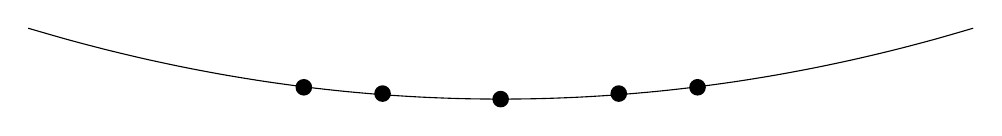
\begin{tikzpicture}
	\draw[scale=2,domain=-3:3,smooth,variable=\x,black] plot ({\x}, {0.05*\x*\x});
	\fill (0, 0) circle[radius=3pt];
	\fill (1.5, 0.07) circle[radius=3pt];
	\fill (-1.5, 0.07) circle[radius=3pt];
	\fill (2.5, 0.15) circle[radius=3pt];
	\fill (-2.5, 0.15) circle[radius=3pt];
\end{tikzpicture}\end{center}
A symmetric catenary bridge forms a U shape. If I some equally-spaced rocks on the bridge, will the average
height be higher or lower than the height of the rock in the middle?
\section{Cauchy-Bunyakovsky-Schwarz Inequality}
For some 2 sequences of real numbers $a_n$ and $b_n$,
\[(a_1^2 + a_2^2 + ... + a_n^2) \cdot (b_1^2 + b_2^2 + ... + b_n^2) \geq (a_1 \cdot b_1 + a_2 \cdot b_2 + ... + a_n \cdot b_n)^2 \]

\section{Arithmetic Mean - Geometric Mean Inequality}
For a sequence $a_n$ of \textbf{non-negative} numbers:
\[\left(a_1 + a_2 + ... + a_n\right) \cdot \frac{1}{n} \geq (a_1 \times a_2 \times  ... \times a_n)^{\frac{1}{n}} \]
\textbf{Practice}

If I have $n$ positive numbers whose product is $1$, what is the minimum possible sum of the numbers?
\end{document}
